\section{Results and Analysis}
\label{sec:results}

After the completion of the experiment programs' development, an automation mechanism was developed based on the GNU Make tool. This mechanism allowed for the repeated running of the experiments suite while also providing control over aspects such as the number of repetitions and grouping of the algorithms.

The basis for the mechanism was a series of additional rules added to the already-present ``Makefile'' files that had been developed for the building of each language's set of programs. A single target-rule, ``\texttt{experiments}'', would recursively descend into each language-specific directory and trigger all algorithms in sequence. Each algorithm ran a specified number of times, and in most cases the initial run was discarded. This was to prevent the possibility of the data input files being in the disk device's cache skewing the timing and energy readings with regards to later runs. All non-error output from the experiments was captured by the harness program and streamed to a single text file.

The format chosen for the file of results was YAML\footnote{YAML: \texttt{https://yaml.org/}}, due to the ready availability of parsing libraries. YAML had an advantage over other formats such as CSV (comma-separated values) in that it allowed the flexibility of complex nested data were it to be necessary, while also being emitted in a streaming fashion. This greatly reduced the potential for output to be corrupted between algorithm executions.

\subsection{Results from the Experiments}
\label{subsec:results}

The automated suite of experiments was run numerous times over the course of this research. The final run from which the analysis and conclusions are drawn is preserved in the same repository on the GitHub platform~\cite{github} as all the other files related to this research. The file of raw experiments data is named ``\texttt{experiments-data-20221104.yml}''.

\subsubsection{Scope of the Experiments}

The final run of the experiments generated a total of 1,190 data-points taken from runs of the 27 programs. Table~\ref{table:iterations} shows the number of runs on a per-language, per-algorithm basis.

\begin{table}[h!]
\begin{center}
% Table: Algorithm iteration counts
% Generated: 2022-11-02 11:35:18.508914
\begin{tabular}{|c|c|c|c|c|c|c|}
\hline
Language&Knuth-Morris-Pratt&Boyer-Moore&Bitap&Aho-Corasick&DFA-Gap&Regexp-Gap \\
\hline
C (GCC)&25&25&25&25&10&n/a \\
C (LLVM)&25&25&25&25&10&n/a \\
C (Intel)&25&25&25&25&10&n/a \\
C++ (GCC)&25&25&25&25&10&n/a \\
C++ (LLVM)&25&25&25&25&10&n/a \\
C++ (Intel)&25&25&25&25&10&n/a \\
Rust&25&25&25&25&10&n/a \\
Perl&5&5&5&25&3&n/a \\
Python&5&5&5&25&3&n/a \\
\hline
\end{tabular}

\caption{Experiment iterations by language and algorithm}
\label{table:iterations}
\end{center}
\end{table}

For all numbers greater than or equal to 10, there was an additional ``priming'' run (as described above) to ensure that disk cache status did not play into the values for full run-time or package-level energy usage. Note also that the DFA-Gap and Regexp-Gap columns are stand-ins for 5 such columns each (for the values of $k$ from 1 to 5). Each value of $k$ was run the same number of iterations.

\subsubsection{Outliers and the Interpreted Languages}

While it was known that the interpreted languages (Python and Perl) would be slower than the compiled languages, the reality of the results was surprising: as will be shown in section~\ref{subsec:perf_comp}, below, the interpreted languages were in some cases more than 150 times slower than the fastest compiled program on the same algorithm.

This discovery required adjusting the automated experiments, to reduce the number of iterations for both interpreted languages. The Knuth-Morris-Pratt, Boyer-Moore, and Bitap algorithms were all reduced to 5 iterations each, for these languages. The Aho-Corasick algorithm ran in a more reasonable length of time and was left at 25 iterations, the same number as were run for the compiled languages.

For the DFA-Gap algorithm, both compiled and interpreted languages had to be reduced in terms of iterations given that approximate-matching algorithms are in general slower than their exact-matching counterparts. The compiled languages ran 10 iterations of this algorithm for values of $k$ ranging from 1 to 5, whereas the interpreted languages were necessarily limited to 3 iterations for the same values of $k$.

\subsection{Performance Comparisons}
\label{subsec:perf_comp}

The collection of sub-tables in table~\ref{table:runtime:comparative-algorithm} shows the comparative performance of the languages on each of the algorithms. The time measurements are based on the algorithm run-time as opposed to the total run-time. In each table, the fastest language is listed first with the remaining ones following in order of performance. Run times are scaled by the fastest time. This has the result of showing each slower language's time as a percentage over the fastest.

\begin{table}[!htb]
% Table: Comparative runtimes sub-tables
% Generated: 2022-11-12 18:00:26.811341
\begin{subtable}{0.33\textwidth}
    \centering
    \caption{Knuth-Morris-Pratt}
    \label{table:runtime:kmp}
    \begin{tabular}{|l|r|}
        %% Caption: Knuth-Morris-Pratt
        %% Label: table:runtime:kmp
        %% Field(s): ['runtime']
        \hline
        Language & Score \\
        \hline
        C (LLVM) & 1.0000 \\
        Rust & 1.1293 \\
        C++ (LLVM) & 1.1377 \\
        C (Intel) & 1.1402 \\
        C++ (Intel) & 1.2406 \\
        C (GCC) & 1.3146 \\
        C++ (GCC) & 1.3350 \\
        Perl & 38.5237 \\
        Python & 41.4858 \\
        \hline
    \end{tabular}
\end{subtable}%
\begin{subtable}{0.33\textwidth}
    \centering
    \caption{Boyer-Moore}
    \label{table:runtime:boyer_moore}
    \begin{tabular}{|l|r|}
        %% Caption: Boyer-Moore
        %% Label: table:runtime:boyer_moore
        %% Field(s): ['runtime']
        \hline
        Language & Score \\
        \hline
        C (Intel) & 1.0000 \\
        C++ (Intel) & 1.0508 \\
        C (GCC) & 1.0664 \\
        Rust & 1.0977 \\
        C++ (LLVM) & 1.1413 \\
        C (LLVM) & 1.1549 \\
        C++ (GCC) & 1.1831 \\
        Perl & 46.9470 \\
        Python & 50.9587 \\
        \hline
    \end{tabular}
\end{subtable}%
\begin{subtable}{0.33\textwidth}
    \centering
    \caption{Bitap}
    \label{table:runtime:shift_or}
    \begin{tabular}{|l|r|}
        %% Caption: Bitap
        %% Label: table:runtime:shift_or
        %% Field(s): ['runtime']
        \hline
        Language & Score \\
        \hline
        C (Intel) & 1.0000 \\
        C (GCC) & 1.0068 \\
        C++ (Intel) & 1.0475 \\
        C (LLVM) & 1.1219 \\
        Rust & 1.1350 \\
        C++ (GCC) & 1.1616 \\
        C++ (LLVM) & 1.2381 \\
        Perl & 155.3435 \\
        Python & 192.9283 \\
        \hline
    \end{tabular}
\end{subtable}
\begin{subtable}{0.33\textwidth}
    \centering
    \caption{Aho-Corasick}
    \label{table:runtime:aho_corasick}
    \begin{tabular}{|l|r|}
        %% Caption: Aho-Corasick
        %% Label: table:runtime:aho_corasick
        %% Field(s): ['runtime']
        \hline
        Language & Score \\
        \hline
        C (LLVM) & 1.0000 \\
        C (Intel) & 1.0443 \\
        C (GCC) & 1.0644 \\
        C++ (GCC) & 1.1519 \\
        C++ (LLVM) & 1.1600 \\
        Rust & 1.1816 \\
        C++ (Intel) & 1.1988 \\
        Python & 19.7040 \\
        Perl & 39.4041 \\
        \hline
    \end{tabular}
\end{subtable}%
\begin{subtable}{0.33\textwidth}
    \centering
    \caption{DFA-Gap (k=3)}
    \label{table:runtime:dfa_gap}
    \begin{tabular}{|l|r|}
        %% Caption: DFA-Gap (k=3)
        %% Label: table:runtime:dfa_gap
        %% Field(s): ['runtime']
        \hline
        Language & Score \\
        \hline
        C (GCC) & 1.0000 \\
        C (LLVM) & 1.0749 \\
        C (Intel) & 1.1561 \\
        C++ (GCC) & 1.2270 \\
        C++ (LLVM) & 1.3250 \\
        C++ (Intel) & 1.3443 \\
        Rust & 1.7632 \\
        Perl & 56.2209 \\
        Python & 57.4437 \\
        \hline
    \end{tabular}
\end{subtable}%
\begin{subtable}{0.33\textwidth}
    \centering
    \caption{Regexp-Gap (k=3)}
    \label{table:runtime:regexp}
    \begin{tabular}{|l|r|}
        %% Caption: Regexp-Gap (k=3)
        %% Label: table:runtime:regexp
        %% Field(s): ['runtime']
        \hline
        Language & Score \\
        \hline
        Rust & 1.0000 \\
        C++ (LLVM) & 1.1747 \\
        C++ (GCC) & 1.1753 \\
        C++ (Intel) & 1.1794 \\
        C (Intel) & 1.2871 \\
        C (GCC) & 1.2876 \\
        C (LLVM) & 1.2888 \\
        Python & 1.7398 \\
        Perl & 3.9966 \\
        \hline
    \end{tabular}
\end{subtable}

\caption{Comparative run-times by algorithm}
\label{table:runtime:comparative-algorithm}
\end{table}

The DFA-Gap algorithm is shown for all values of $k$ that were used, as it is interesting to see the subtle differences in the ranking of languages for different values of $k$.

\subsection{Energy Usage Comparisons}
\label{subsec:energy_comp}

In this section the energy usage results are examined. Table~\ref{table:energy:comparative-algorithm} shows the comparative energy usage over time (Joules per second) for each algorithm with the same scaling methodology applied as was used for the performance tables. The tables here use the ``Package'' and ``DRAM'' energy values combined together, divided by total run-time.

\begin{table}[!htb]
% Table: Comparative energy usage sub-tables
% Generated: 2022-11-11 19:03:08.364288
\begin{subtable}{0.33\textwidth}
    \centering
    \caption{Knuth-Morris-Pratt}
    \label{table:energy:kmp}
    \begin{tabular}{|l|r|}
        %% Caption: Knuth-Morris-Pratt
        %% Label: table:energy:kmp
        %% Field(s): ['package', 'dram']
        %% Divisor(s): ['total_runtime']
        \hline
        Language & Score \\
        \hline
        Rust & 1.0000 \\
        C (GCC) & 1.0403 \\
        C (LLVM) & 1.0756 \\
        C (Intel) & 1.0786 \\
        C++ (GCC) & 1.0983 \\
        C++ (LLVM) & 1.1033 \\
        C++ (Intel) & 1.1102 \\
        Python & 1.1651 \\
        Perl & 1.2957 \\
        \hline
    \end{tabular}
\end{subtable}%
\begin{subtable}{0.33\textwidth}
    \centering
    \caption{Boyer-Moore}
    \label{table:energy:boyer_moore}
    \begin{tabular}{|l|r|}
        %% Caption: Boyer-Moore
        %% Label: table:energy:boyer_moore
        %% Field(s): ['package', 'dram']
        %% Divisor(s): ['total_runtime']
        \hline
        Language & Score \\
        \hline
        C++ (GCC) & 1.0000 \\
        C++ (LLVM) & 1.0115 \\
        Rust & 1.0331 \\
        C (GCC) & 1.0358 \\
        C++ (Intel) & 1.0747 \\
        C (LLVM) & 1.0918 \\
        C (Intel) & 1.1501 \\
        Python & 1.2985 \\
        Perl & 1.3103 \\
        \hline
    \end{tabular}
\end{subtable}%
\begin{subtable}{0.33\textwidth}
    \centering
    \caption{Bitap}
    \label{table:energy:shift_or}
    \begin{tabular}{|l|r|}
        %% Caption: Bitap
        %% Label: table:energy:shift_or
        %% Field(s): ['package', 'dram']
        %% Divisor(s): ['total_runtime']
        \hline
        Language & Score \\
        \hline
        C++ (LLVM) & 1.0000 \\
        C (Intel) & 1.0049 \\
        Rust & 1.0077 \\
        C (LLVM) & 1.0101 \\
        C++ (Intel) & 1.0440 \\
        Python & 1.0799 \\
        C++ (GCC) & 1.0854 \\
        C (GCC) & 1.0897 \\
        Perl & 1.2268 \\
        \hline
    \end{tabular}
\end{subtable}
\begin{subtable}{0.33\textwidth}
    \centering
    \caption{Aho-Corasick}
    \label{table:energy:aho_corasick}
    \begin{tabular}{|l|r|}
        %% Caption: Aho-Corasick
        %% Label: table:energy:aho_corasick
        %% Field(s): ['package', 'dram']
        %% Divisor(s): ['total_runtime']
        \hline
        Language & Score \\
        \hline
        C++ (LLVM) & 1.0000 \\
        C (Intel) & 1.0303 \\
        C (GCC) & 1.0332 \\
        C (LLVM) & 1.0448 \\
        C++ (Intel) & 1.0471 \\
        C++ (GCC) & 1.0813 \\
        Rust & 1.0939 \\
        Perl & 1.1248 \\
        Python & 1.1736 \\
        \hline
    \end{tabular}
\end{subtable}%
\begin{subtable}{0.33\textwidth}
    \centering
    \caption{DFA-Gap (k=3)}
    \label{table:energy:dfa_gap(3)}
    \begin{tabular}{|l|r|}
        %% Caption: DFA-Gap (k=3)
        %% Label: table:energy:dfa_gap(3)
        %% Field(s): ['package', 'dram']
        %% Divisor(s): ['total_runtime']
        \hline
        Language & Score \\
        \hline
        Rust & 1.0000 \\
        C++ (LLVM) & 1.1603 \\
        C (LLVM) & 1.1812 \\
        C++ (Intel) & 1.2078 \\
        C (Intel) & 1.2231 \\
        C (GCC) & 1.2352 \\
        C++ (GCC) & 1.2497 \\
        Python & 1.3140 \\
        Perl & 1.3897 \\
        \hline
    \end{tabular}
\end{subtable}%
\begin{subtable}{0.33\textwidth}
    \centering
    \caption{Regexp-Gap (k=3)}
    \label{table:energy:regexp(3)}
    \begin{tabular}{|l|r|}
        %% Caption: Regexp-Gap (k=3)
        %% Label: table:energy:regexp(3)
        %% Field(s): ['package', 'dram']
        %% Divisor(s): ['total_runtime']
        \hline
        Language & Score \\
        \hline
        C (Intel) & 1.0000 \\
        C (GCC) & 1.0055 \\
        C (LLVM) & 1.0094 \\
        C++ (LLVM) & 1.0428 \\
        C++ (GCC) & 1.0460 \\
        C++ (Intel) & 1.0473 \\
        Perl & 1.0513 \\
        Rust & 1.0561 \\
        Python & 1.0618 \\
        \hline
    \end{tabular}
\end{subtable}

\caption{Comparative energy usage over time by algorithm}
\label{table:energy:comparative-algorithm}
\end{table}

The language exhibiting the lowest energy usage is listed first, with the rest ranked behind it. The DFA-Gap algorithm is again represented for all values of $k$, as the ranking of languages varies with $k$.

These results are further illustrated by figure~\ref{fig:graph:power_per_sec}. In this collection of bar-charts, the Rust language (represented by the pink bars) can be seen to be the lowest value in the Knuth-Morris-Pratt, Boyer-Moore, and DFA-Gap ($k=1$) instances. In fact, Rust scored the lowest energy usage for all five variations of the DFA-Gap algorithm, making it the most-efficient language for 7 of the 9 distinct groups of experiments.

\begin{figure}
	\centering
	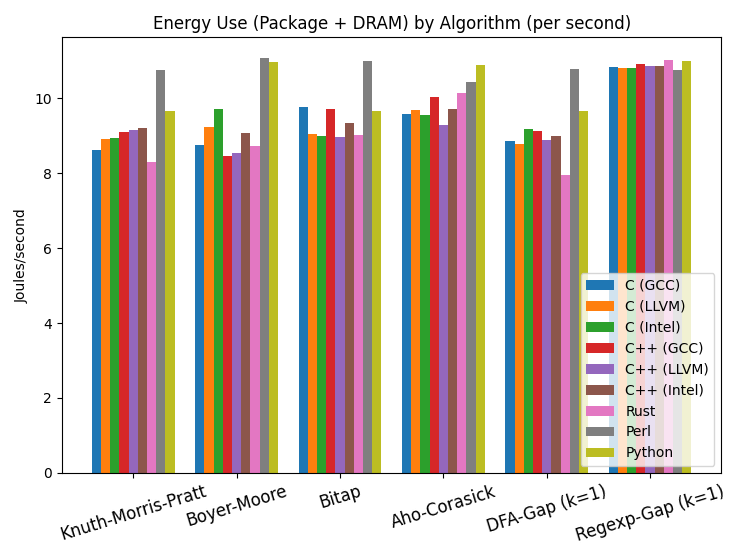
\includegraphics[width=0.85\textwidth]{figures/power_per_sec.png}
	\caption{Bar charts of energy usage per second, by algorithm}
	\label{fig:graph:power_per_sec}
\end{figure}

\subsection{Expressiveness Comparisons}
\label{subsec:expr_comp}

In comparing expressiveness, it is useful to look at all three of the chosen comparative measures in an aggregated fashion. First, the individual numbers will be examined. As with the previous two bases, tables will show the numbers comparing the languages. Unlike the previous sections, the numbers shown will be for the combined files of all algorithm modules, as well as runner modules and input modules. For each language the source code was combined in a way that facilitated each of the metrics:

\begin{description}
\item[SLOC:] Total SLOC values for each language's files were combined. In the case of C and C++, this includes relevant lines from the header files for the runner and input modules.
\item[Complexity:] Each file's cyclomatic complexity values were computed on a per-function basis. Any function whose value was exactly 1 was discarded so as to not artificially lower the average complexity for the module. Each module's function-level scores were then averaged, and all modules' averages for a given language were summed together.
\item[Conciseness:] Using a method identical to Bergmans, et al~\cite{bergmans}, each source code file for a given language was stripped of comments and then archived together using the standard ``\texttt{tar}'' command available on Linux. Each archive file was then compressed with the ``\texttt{xz}'' compression utility and the compression ratio recorded.
\end{description}

\subsubsection{Source Lines of Code}

\begin{table}[!htb]
% Table: Comparative SLOC totals sub-tables
% Generated: 2022-11-04 19:01:11.807483
\begin{subtable}{0.33\textwidth}
    \centering
    \begin{tabular}{|c|r|r|}
        \hline
        Language & Code & Score \\
        \hline
        Python & 257 & 1.0000 \\
        Perl & 354 & 1.3774 \\
        C++ & 368 & 1.4319 \\
        C & 473 & 1.8405 \\
        Rust & 507 & 1.9728 \\
        \hline
    \end{tabular}
    \caption{Algorithm lines}
    \label{table:sloc:algorithm}
\end{subtable}%
\begin{subtable}{0.33\textwidth}
    \centering
    \begin{tabular}{|c|r|r|}
        \hline
        Language & Support & Score \\
        \hline
        Python & 148 & 1.0000 \\
        Perl & 211 & 1.4257 \\
        C++ & 266 & 1.7973 \\
        Rust & 272 & 1.8378 \\
        C & 353 & 2.3851 \\
        \hline
    \end{tabular}
    \caption{Framework lines}
    \label{table:sloc:framework}
\end{subtable}%
\begin{subtable}{0.33\textwidth}
    \centering
    \begin{tabular}{|c|r|r|}
        \hline
        Language & All & Score \\
        \hline
        Python & 405 & 1.0000 \\
        Perl & 565 & 1.3951 \\
        C++ & 634 & 1.5654 \\
        Rust & 779 & 1.9235 \\
        C & 826 & 2.0395 \\
        \hline
    \end{tabular}
    \caption{Total of lines}
    \label{table:sloc:all}
\end{subtable}

\caption{Comparison of SLOC by language}
\label{table:expr:sloc}
\end{table}

\subsubsection{Cyclomatic Complexity}

\begin{table}[!htb]
% Table: Comparative cyclomatic totals sub-tables
% Generated: 2022-11-12 18:00:26.813913
\begin{subtable}{0.33\textwidth}
    \centering
    \caption{Algorithms complexity}
    \label{table:cyclomatic:algorithm}
    \begin{tabular}{|c|r|r|}
        \hline
        Language & Total & Avg \\
        \hline
        Python & 76 & 19.57 \\
        C++ & 81 & 16.83 \\
        Perl & 106 & 26.97 \\
        C & 114 & 18.30 \\
        Rust & 132 & 17.97 \\
        \hline
    \end{tabular}
\end{subtable}%
\begin{subtable}{0.33\textwidth}
    \centering
    \caption{Framework complexity}
    \label{table:cyclomatic:framework}
    \begin{tabular}{|c|r|r|}
        \hline
        Language & Total & Avg \\
        \hline
        C++ & 43 & 10.75 \\
        Python & 47 & 9.90 \\
        Rust & 58 & 5.43 \\
        Perl & 61 & 12.90 \\
        C & 76 & 19.00 \\
        \hline
    \end{tabular}
\end{subtable}%
\begin{subtable}{0.33\textwidth}
    \centering
    \caption{Total complexity}
    \label{table:cyclomatic:total}
    \begin{tabular}{|c|r|r|}
        \hline
        Language & Total & Avg \\
        \hline
        Python & 123 & 29.47 \\
        C++ & 124 & 27.58 \\
        Perl & 167 & 39.87 \\
        C & 190 & 37.30 \\
        Rust & 190 & 23.40 \\
        \hline
    \end{tabular}
\end{subtable}

\caption{Comparison of complexity by language}
\label{table:expr:cyclomatic}
\end{table}

\subsubsection{Conciseness}

\begin{table}[!htb]
% Table: Compression ratios table
% Generated: 2022-11-11 19:03:08.366214
\centering
\begin{tabular}{|l|c|c|}
    \hline
    Language & Ratio & Score \\
    \hline
    Python & 78.50\% & 1.0000 \\
    Perl & 80.50\% & 1.0255 \\
    C & 80.60\% & 1.0268 \\
    Rust & 80.80\% & 1.0293 \\
    C++ & 81.00\% & 1.0318 \\
    \hline
\end{tabular}

\caption{Comparison of compressibility}
\label{table:expr:compression}
\end{table}

\subsection{Combined Bases}
\label{subsec:combined}
